\documentclass[12pt]{article}
\usepackage{times}
\usepackage[english]{babel}
\usepackage[utf8x]{inputenc}
\usepackage[colorinlistoftodos]{todonotes}
\usepackage[margin=1in]{geometry}
\usepackage{graphicx}
\usepackage{epstopdf}
\usepackage{cite}
\usepackage{listings}
\usepackage{dtklogos}
\usepackage{wrapfig}
\usepackage{subfigure}
\usepackage{amsmath}
\usepackage{amsthm}
\usepackage{amssymb}
\usepackage{amscd}
\usepackage{caption}
\usepackage{etoolbox}
\usepackage{fancyhdr}
\usepackage{stackengine}
\usepackage[export]{adjustbox}
\usepackage{rotating}
\patchcmd{\thebibliography}{\section*{\refname}}{}{}{}
\usepackage[document]{ragged2e}    %This causes text to left align
\usepackage[colorlinks=true, linkcolor=black,citecolor=black,urlcolor=blue]{hyperref}
\bibliographystyle{IEEEtran}
\extrafloats{100}
\DeclareGraphicsRule{.tif}{png}{.png}{`convert #1 `dirname #1`/`basename #1 .tif`.png}

\title{MCHE 357: Lab 10}

\begin{document}
\lefthyphenmin3
\righthyphenmin4
% \pretolerance=2000
% \tolerance=500 
% \emergencystretch=10pt
%\raggedright     %Stops LaTeX from automatically hyphenating the right margin to fit better
%Combine this with \usepackage[document]{ragged2e} to get a text align left similar to natural MS Word


%-------------------------------------------------------------
%Start of Paper
%-------------------------------------------------------------

%%%%%%%%%%%%%%%%%%%%%%%%%%%%%%%%%%%%%%%%%%%%%%%%%%%%%%
%%%%%%%%%%%%%%%%%%%%%%% TITLE PAGE %%%%%%%%%%%%%%%%%%%%%%%%
%%%%%%%%%%%%%%%%%%%%%%%%%%%%%%%%%%%%%%%%%%%%%%%%%%%%%%

\begin{titlepage}

\newcommand{\HRule}{\rule{\linewidth}{0.5mm}} % Defines a new command for the horizontal lines, change thickness here

\center % Center everything on the page
 
%----------------------------------------------------------------------------------------
%	Heading Section
%----------------------------------------------------------------------------------------

\textsc{\LARGE University of Louisiana at Lafayette}\\[1.5cm] % Name of your university/college
\textsc{\Large Measurements and Instrumentation}\\[0.5cm] % Major heading such as course name
\textsc{\large MCHE 357}\\[0.5cm] % Minor heading such as course title

%----------------------------------------------------------------------------------------
%	Title Section
%----------------------------------------------------------------------------------------

\HRule \\[0.4cm]
{ \huge \bfseries Lab 10}\\[0.4cm] % Title of your document
\HRule \\[1.5cm]
 
%----------------------------------------------------------------------------------------
%	Author Section
%----------------------------------------------------------------------------------------

\begin{minipage}{0.4\textwidth}
\begin{flushleft} \large
\emph{Author:}\\
\textsc{Matthew J. Begneaud} \\% Your name
\end{flushleft}
\end{minipage}
~
\begin{minipage}{0.4\textwidth}
\begin{flushright} \large
\emph{Professor:} \\
\textsc{Dr. Mostafa A. Elsayed} % Supervisor's Name
\end{flushright}
\end{minipage}\\[1.5cm]

% If you don't want a supervisor, uncomment the two lines below and remove the section above
%\Large \emph{Author:}\\
%John \textsc{Smith}\\[3cm] % Your name

%----------------------------------------------------------------------------------------
%	Date Section
%----------------------------------------------------------------------------------------

{\textsc{\large \today}}\\[0.5cm] % Date, change the \today to a set date if you want to be precise


%----------------------------------------------------------------------------------------
%	Group Section
%----------------------------------------------------------------------------------------
\textsc{\large Group:}\\[0.1cm]
\textsc{Ronald Kisor}\\
\textsc{Chandler Lagarde}\\
\textsc{Somto Umeokafor}
\\[0.5cm]

%----------------------------------------------------------------------------------------
%	Logo Section
%----------------------------------------------------------------------------------------


\includegraphics[width=5in]{UL_logo.jpg}\\[1cm] % Include a department/university logo - this will require the graphicx package
 
%----------------------------------------------------------------------------------------

\vfill % Fill the rest of the page with whitespace

\end{titlepage}

%%%%%%%%%%%%%%%%%%%%%%%%%%%%%%%%%%%%%%%%%%%%%%%%%%%%%%
%%%%%%%%%%%%%%%%%%%%%%% TABLE OF CONTENTS %%%%%%%%%%%%%%%%%%%
%%%%%%%%%%%%%%%%%%%%%%%%%%%%%%%%%%%%%%%%%%%%%%%%%%%%%%

\tableofcontents

\listoffigures

\bigskip


\section*{\fontsize{12}{12}\selectfont \large List of Symbols}
\addcontentsline{toc}{section}{List of Symbols} % Add for each section
None




\newpage

%%%%%%%%%%%%%%%%%%%%%%%%%%%%%%%%%%%%%%%%%%%%%%%%%%%%%%
%%%%%%%%%%%%%%%%%%%%%%% REPORT %%%%%%%%%%%%%%%%%%%%%%%%%%
%%%%%%%%%%%%%%%%%%%%%%%%%%%%%%%%%%%%%%%%%%%%%%%%%%%%%%


\section*{\fontsize{12}{12}\selectfont \large Introduction}
\addcontentsline{toc}{section}{Introduction} % Add for each section

This lab consisted of using Labview to create a program which reads data from a strain gauge to measure the stress placed on an object. The program was used to measure the stress on a cantilever beam, as well as its natural frequency.


\section*{\fontsize{12}{12}\selectfont \large Theory}
\addcontentsline{toc}{section}{Theory} % Add for each section

Labview can be used in conjunction with physical instruments in order to control a system or take data in from a system. Reading data from an instrument can be done by referring to the documentation of the instrument in order to map voltage readings to the desired measurement, while also considering the sensitivity of the instrument. 
\bigskip

A strain gauge is a device used to measure stress placed on a material which changes resistance as its elongation changes. This changing resistance results in different voltages being outputted by the device which can then be mapped to stresses. The mean voltage outputted at different stresses is correlated to a stress with a gauge factor. 
\bigskip

\section*{\fontsize{12}{12}\selectfont \large Procedure \& Analysis}
\addcontentsline{toc}{section}{Procedure \& Analysis} % Add for each section

The program used in this lab would read the voltage outputted by the strain gauge and map it to a stress value by use of a gauge factor tabulated in the instrument's documentation. The system diagram and control panel for the Labview program can be seen in Figure 1 and Figure 2, respectively. The data mentioned throughout this section can be seen tabulated in Figure 3. 
\bigskip

A cantilever beam was set up as shown in Figure 4. The gauge was first zeroed out to compensate for the voltage reading when no strain is placed on the gauge. The natural frequency of the cantilever beam was then measured by deflecting the beam and then releasing it, allowing it to oscillate for one second and recording the oscillation data. The frequency was estimated as 17 Hz by plotting the data, shown in Figure 5.
\bigskip
 
A known weight was then hung from the end of the beam to place a load on the beam as shown in Figure 6. The stress caused by this load was recorded. A second weight was then added to the first weight and the stress reading was recorded again. The process was then repeated for a third weight. Between adding weights, the weights were removed momentarily to zero out the gauge again since excessive deflection can change the resting voltage value of the gauge. The data can be seen tabulated by referring back to Figure 3, and the data is plotted in Figure 7. As is expected, the data for the readings is approximately linear as it should be when considering that moments due to a static, concentrated load are linearly proportional to the loading force.
\bigskip

\newpage

\begin{figure}[h!] %  figure placement: here, top, bottom, or page
   \centering
   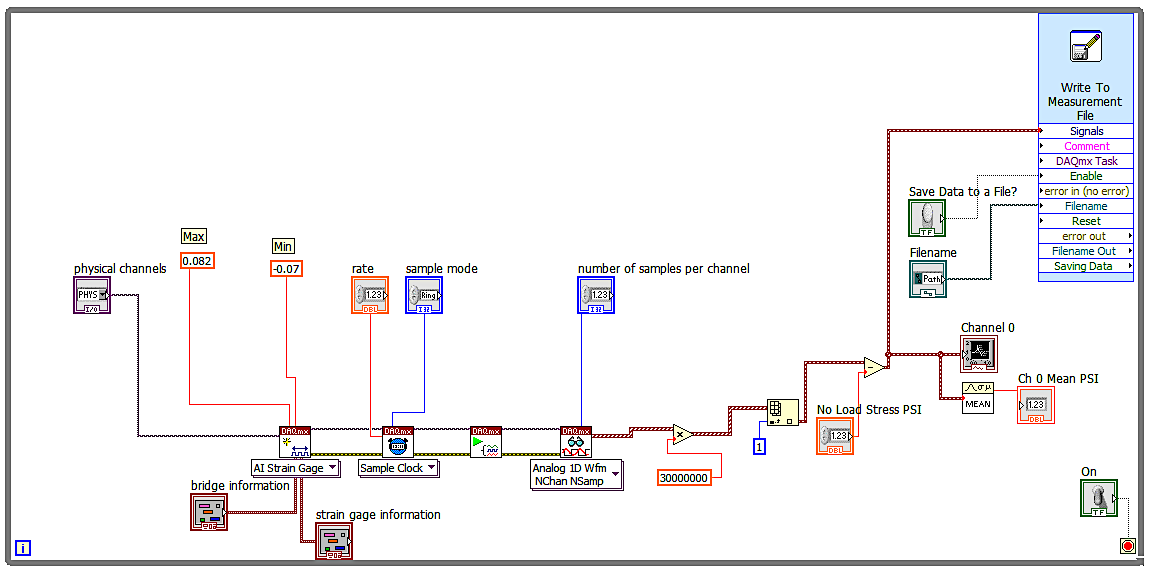
\includegraphics[width=5.5in, height=3.5in]{lab10vi.png} 
   \caption{Labview Program System Diagram}
   \label{fig:example}
\end{figure}

\bigskip
\bigskip

\begin{figure}[h!] %  figure placement: here, top, bottom, or page
   \centering
   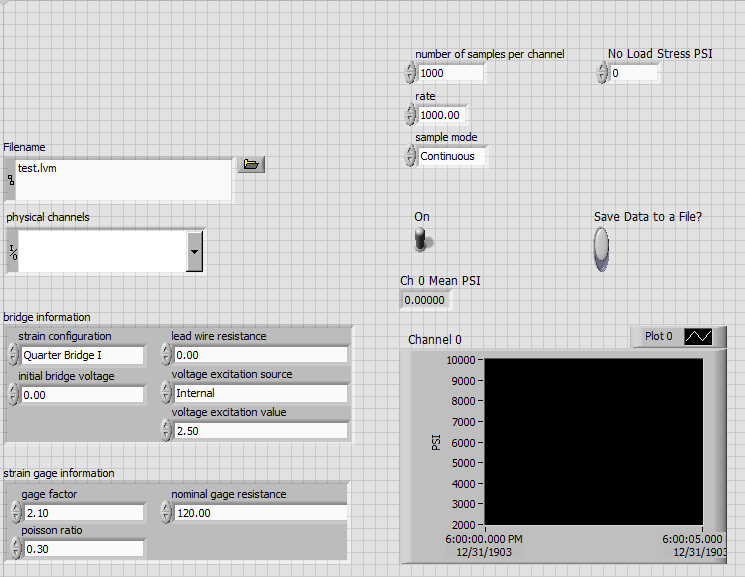
\includegraphics[width=5in]{lab10bd.png} 
   \caption{Labview Program System Control Panel}
   \label{fig:example}
\end{figure}

\newpage

\begin{figure}[h!] %  figure placement: here, top, bottom, or page
   \centering
   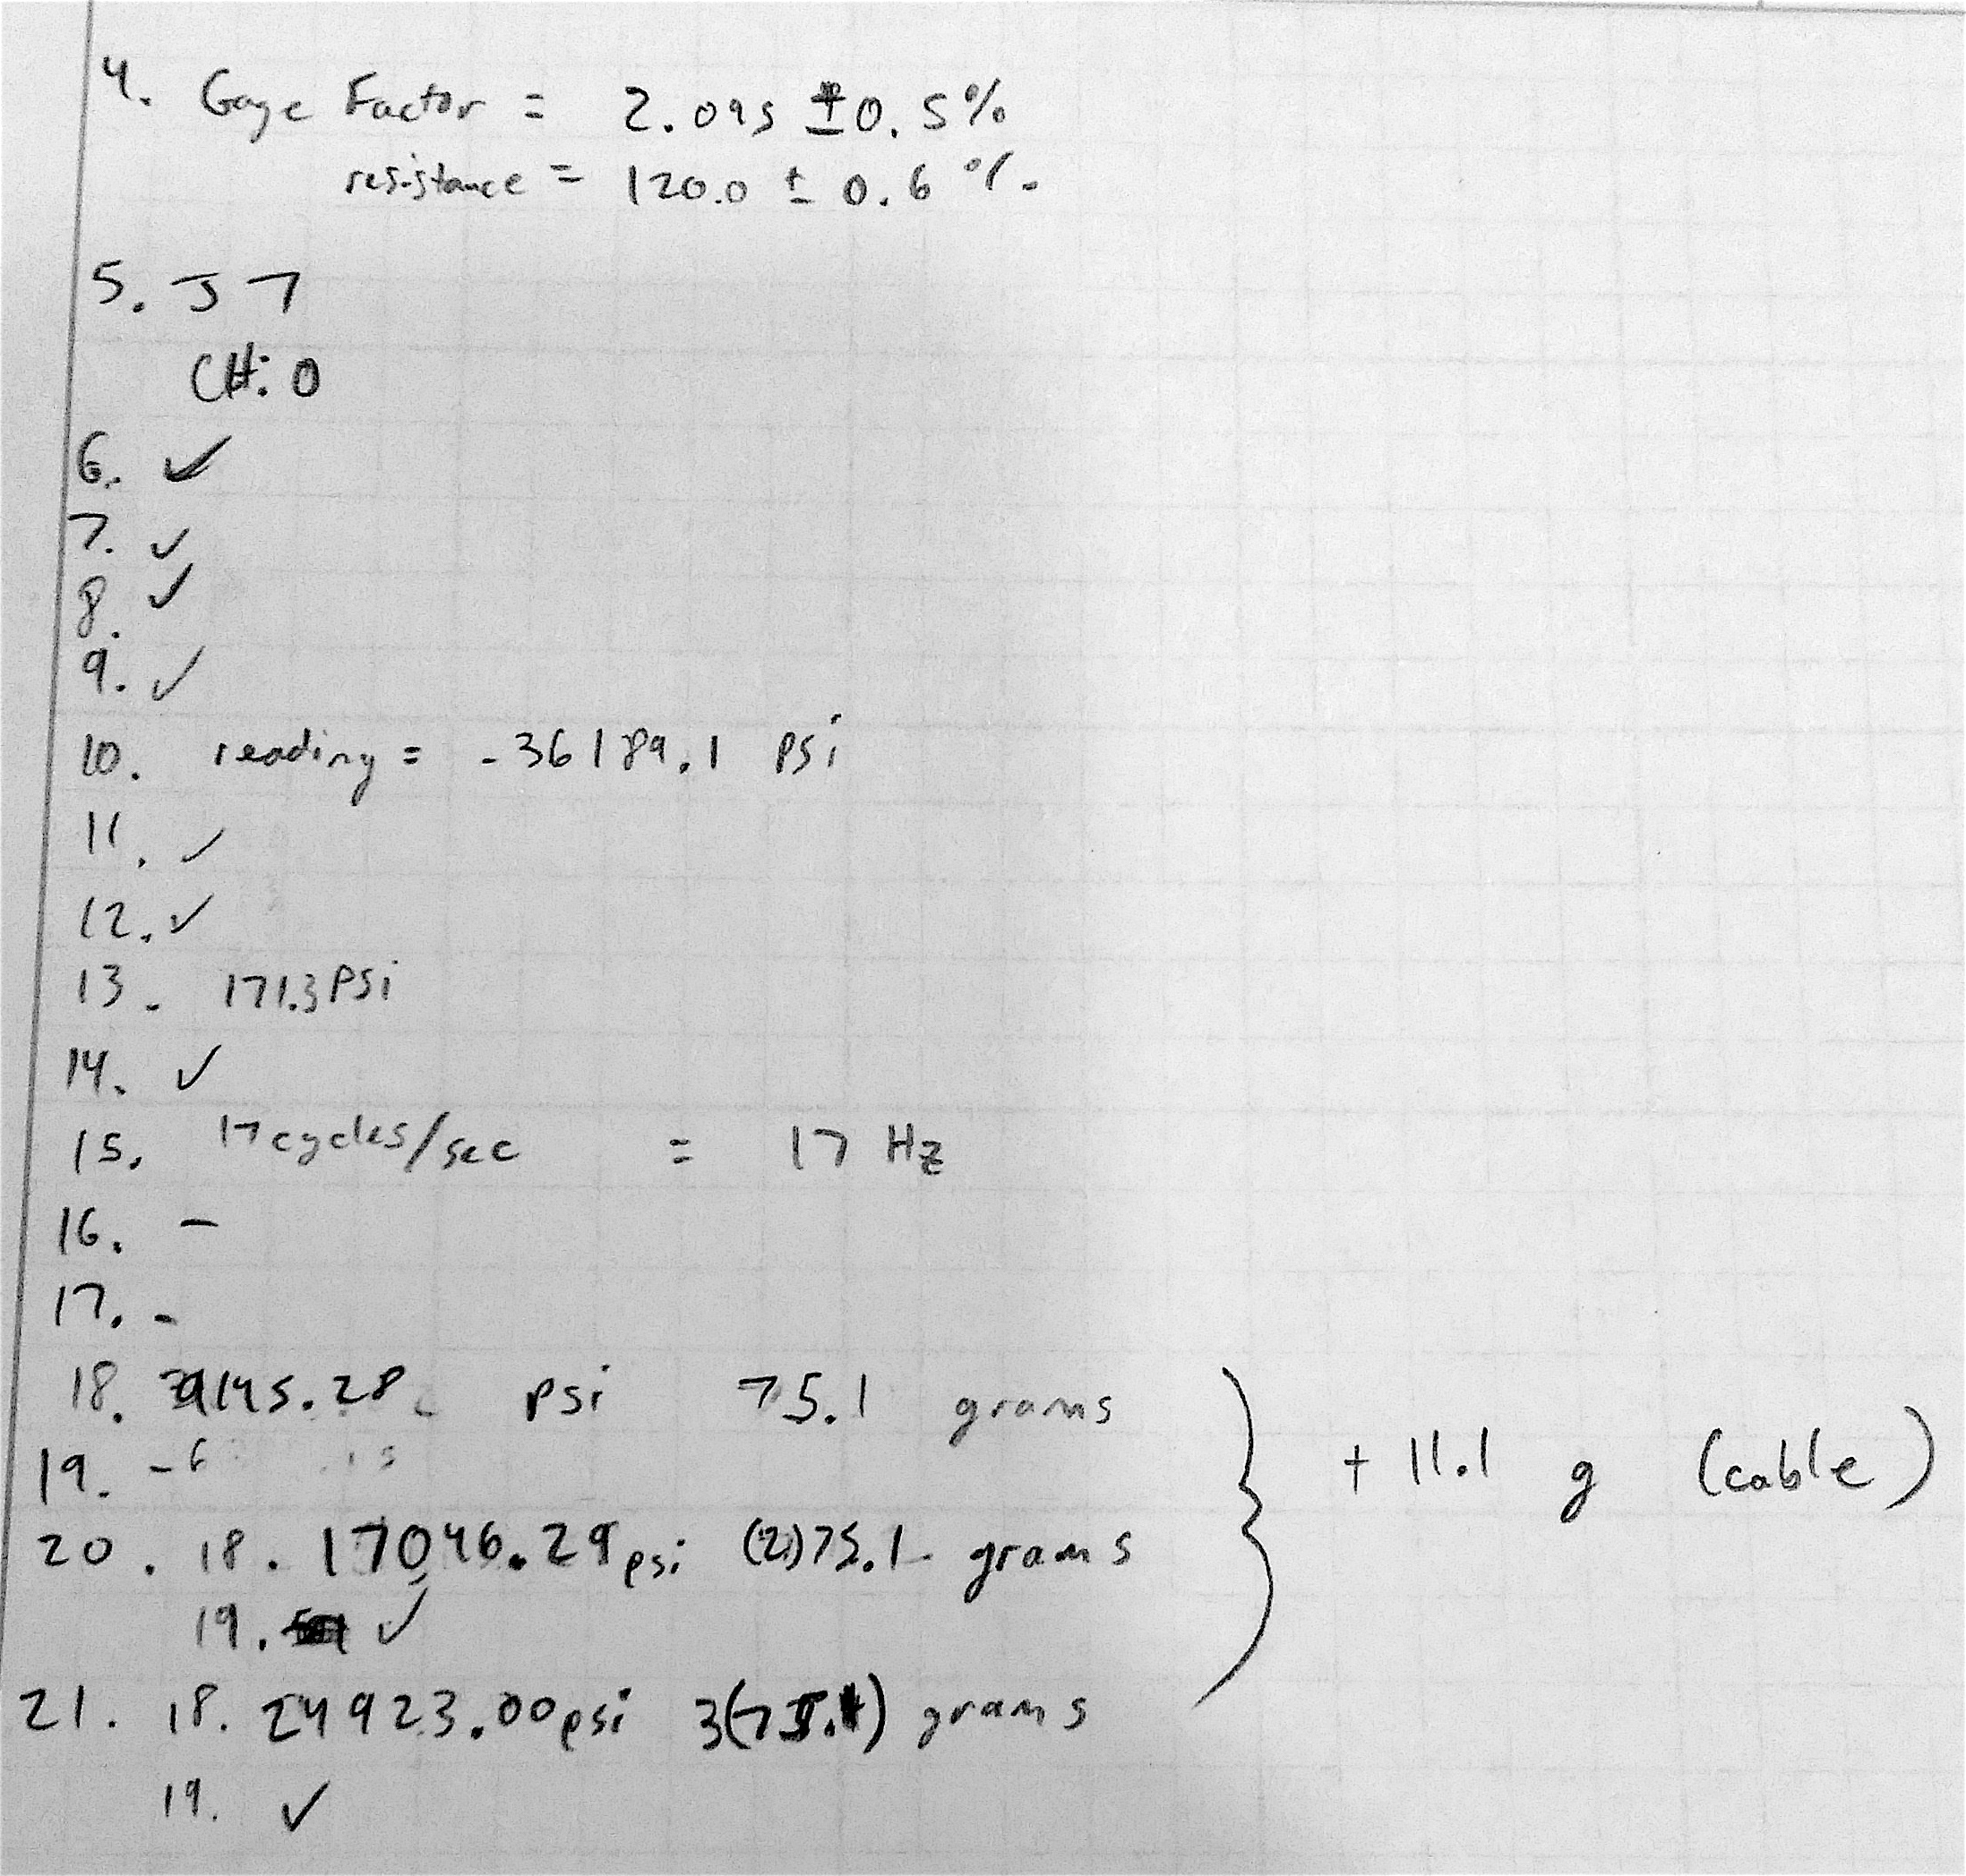
\includegraphics[width=5in]{lab_10_notes.jpg} 
   \caption{Lab Notes}
   \label{fig:example}
\end{figure}

\begin{figure}[h!] %  figure placement: here, top, bottom, or page
   \centering
   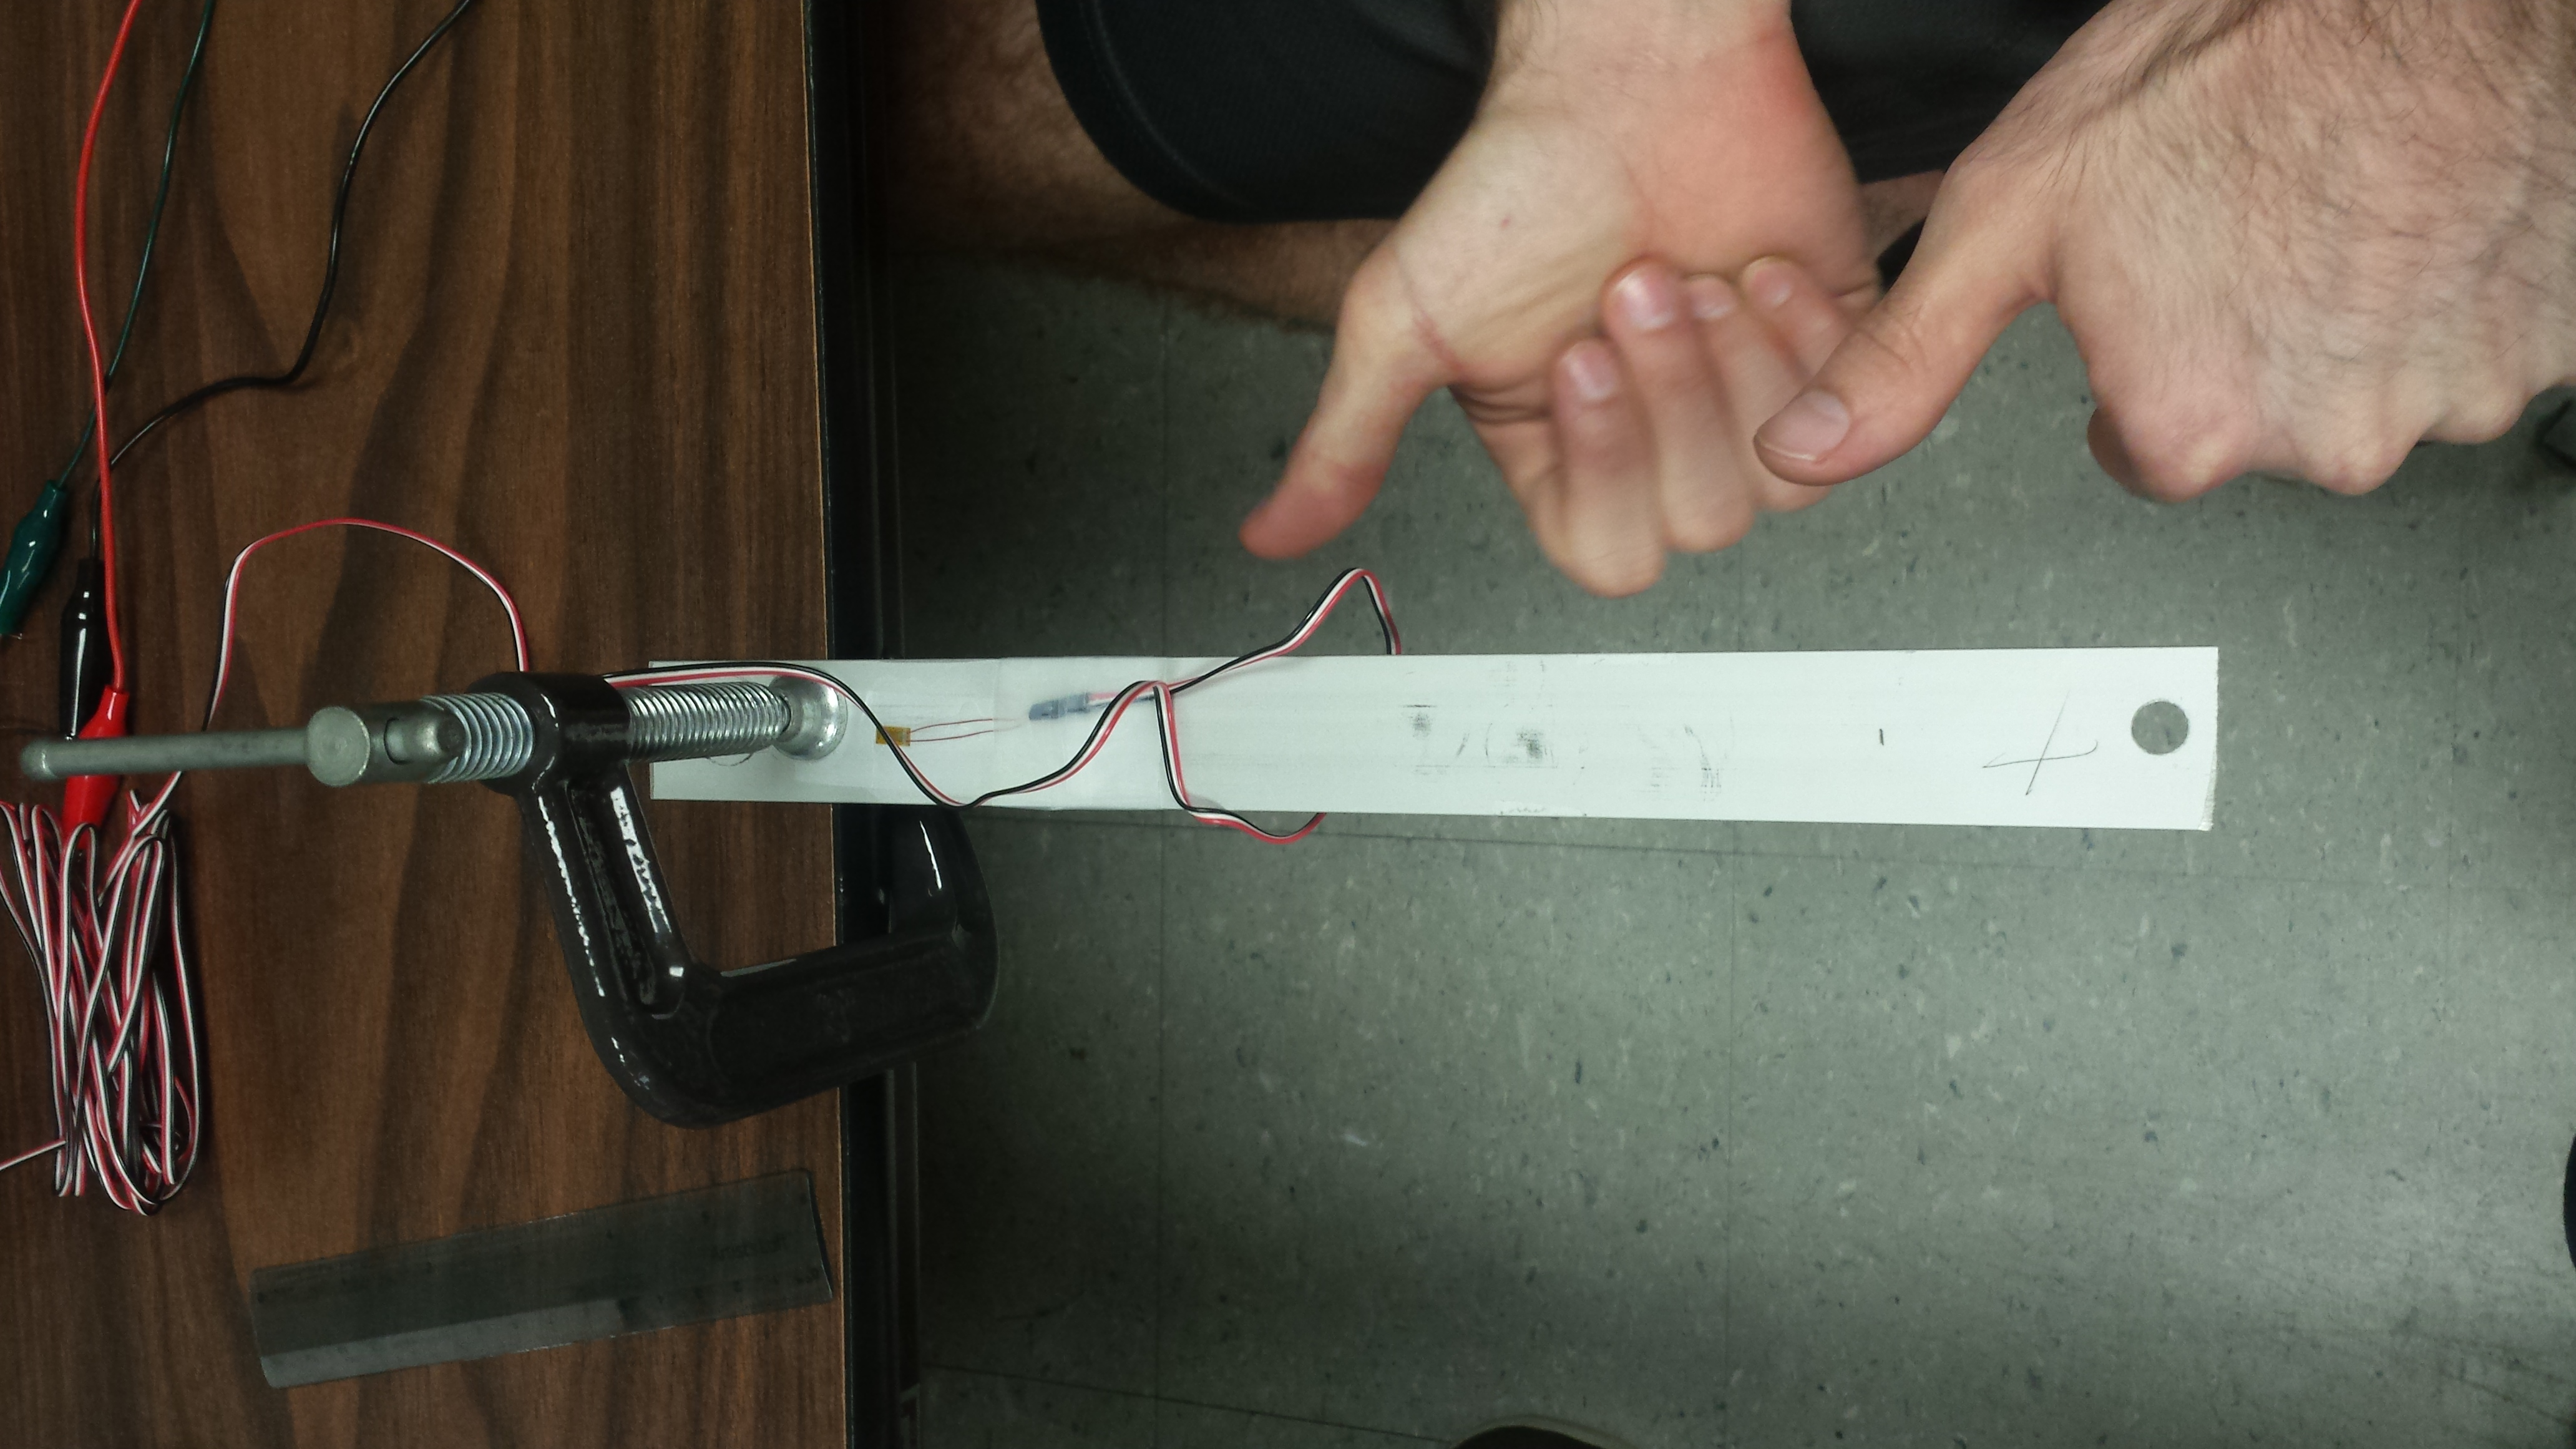
\includegraphics[width=5in]{cantilever_beam.jpg} 
   \caption{Cantilever Beam}
   \label{fig:example}
\end{figure}

\newpage

\begin{figure}[h!] %  figure placement: here, top, bottom, or page
   \centering
   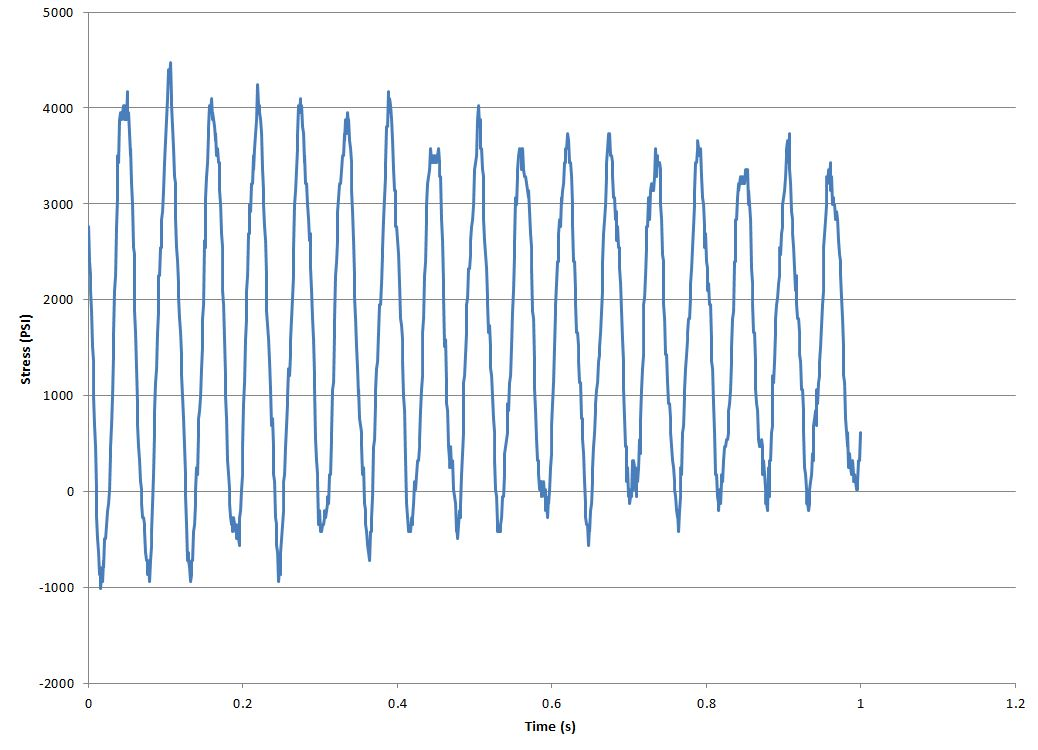
\includegraphics[width=5.5in]{nat_freq_plot.jpg} 
   \caption{Oscillation Data Plot}
   \label{fig:example}
\end{figure}

\bigskip

\begin{figure}[h!] %  figure placement: here, top, bottom, or page
   \centering
   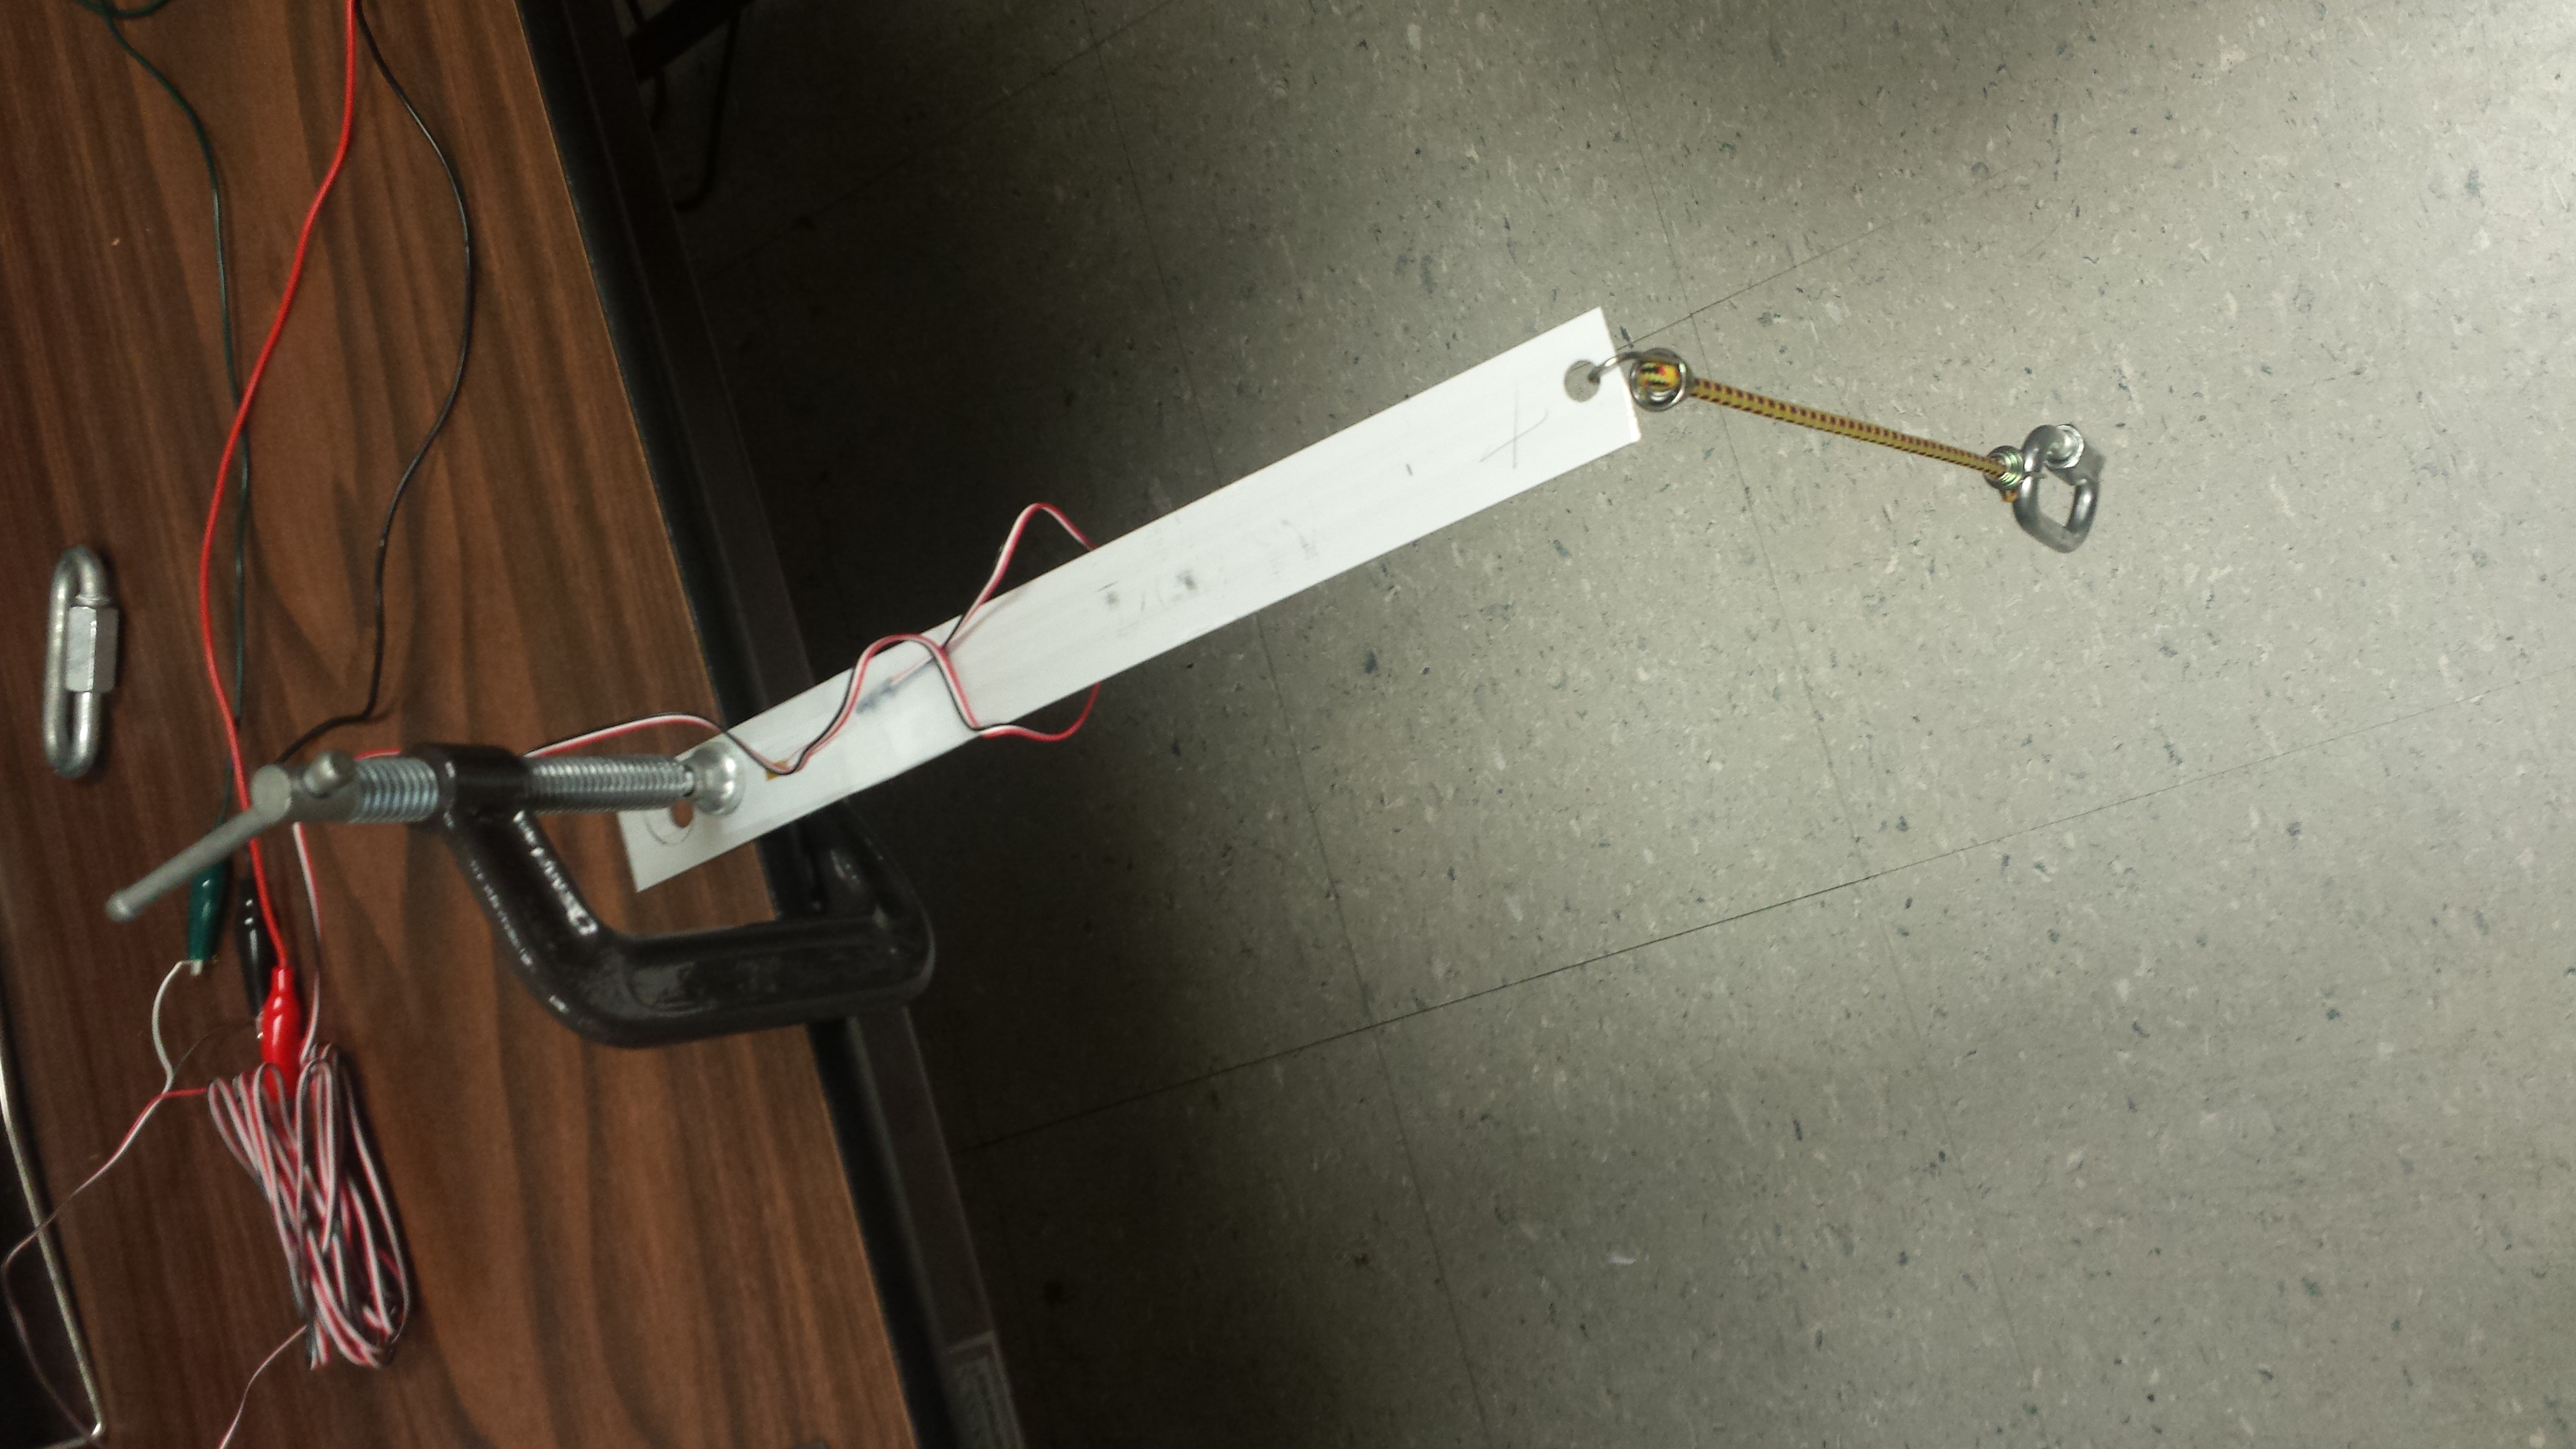
\includegraphics[width=5.5in]{hanging_weight.jpg} 
   \caption{Hanging Weight End-Load}
   \label{fig:example}
\end{figure}

\newpage

\begin{figure}[h!] %  figure placement: here, top, bottom, or page
   \centering
   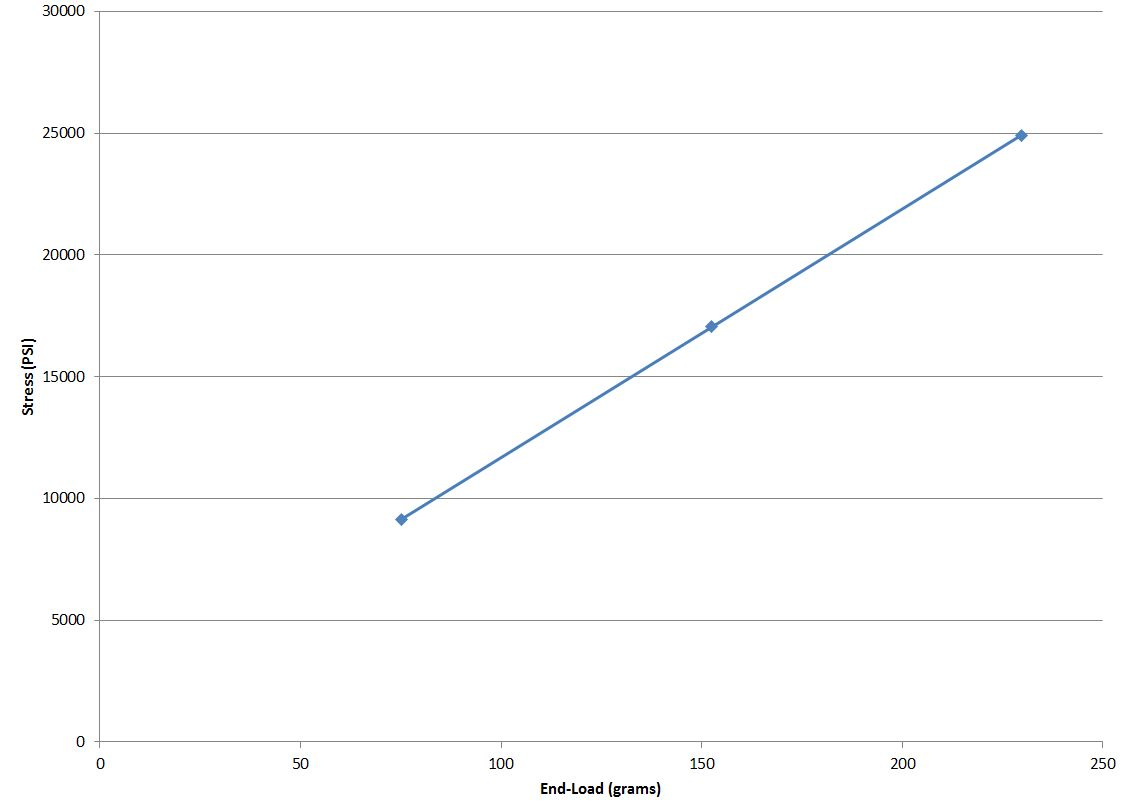
\includegraphics[width=5.5in]{hanging_weight_plot.jpg} 
   \caption{Hanging Weight End-Load Data Plot}
   \label{fig:example}
\end{figure}


\section*{\fontsize{12}{12}\selectfont \large Conclusion}
\addcontentsline{toc}{section}{Conclusion} % Add for each section
The exercises conducted in this lab demonstrated using a Labview program to acquire data. It was shown that reading data from sensors is typically done by mapping the voltage reading from the sensor to a measurement value by using documentation on the specific sensor being used. This is how most measurement systems work, and it is important that students are exposed to using these sensors as they will likely use them in their careers in the industry. Exhibiting this method by measuring something mechanical engineering students are familiar with helps them appreciate the importance of accurate instrumentation in order to acquire accurate data for their work.


%\section*{\fontsize{12}{12}\selectfont \large References}

%\begin{thebibliography}{2}
%
%% Example
%%\bibitem{Wagner}
%%Ng, K., Wagner, S.W., Camelio, J., Emblom, W.J. (2010). ?Experimental Analysis of Micro Tube
%%Hydroforming Process.? Transactions of NAMRC of SME, 38, 577-584.
%
%\end{thebibliography}



%\section*{\fontsize{12}{12}\selectfont APPENDIX}

%\begin{table}[h!]
%  \caption{}
%  \includegraphics[width=\linewidth]{table1.png}
%\end{table}




\end{document}







----------------------------Templates-------------------------------

-------------------------Figure-----------------------

\begin{figure}[h!]  
  \centering
    \includegraphics[width=\linewidth]{**file**}
    \caption{Docking Station}
\end{figure}

---------------------------Table-----------------------
\begin{table}[ht]
\caption{Nonlinear Model Results} % title of Table
\centering % used for centering table
\begin{tabular}{c c c c} % centered columns (4 columns)
\hline\hline %inserts double horizontal lines
Case & Method\#1 & Method\#2 & Method\#3 \\ [0.5ex] % inserts table
%heading
\hline % inserts single horizontal line
1 & 50 & 837 & 970 \\ % inserting body of the table
2 & 47 & 877 & 230 \\
3 & 31 & 25 & 415 \\
4 & 35 & 144 & 2356 \\
5 & 45 & 300 & 556 \\ [1ex] % [1ex] adds vertical space
\hline %inserts single line
\end{tabular}
\label{table:nonlin} % is used to refer this table in the text
\end{table}



probably best to insert as an image from excel

\bigskip\\
\begin{table}[h!]
  \caption{}
  \includegraphics[width=\linewidth]{**file**}
\end{table}
\bigskip\\





-----------------------------Equations------------------------
-----------------------------Regular
\begin{equation}
a = b + c
\end{equation}

--------------------------------- Multiline
\begin{multline}
a = b + c + d + e + f
+ g + h + i + j \\
+ k + l + m + n + o
\end{multline}

-------------------------------Citations-------------------------
\bibitem{Author last name}
  Last, First., year of publication,
  article name, book(etc) name, from \\
  link goes here

----------------------------------other-----------------------------

equations:
http://moser-isi.ethz.ch/docs/typeset_equations.pdf

citations:
http://library.missouri.edu/engineering/about/guides/asme
https://www.asme.org/shop/proceedings/conference-publications/references